\section{Study guide  for ``Permutations''  chapter}\label{sec:Permutations:study} 


\subsection*{Section \ref{introduction}, Introduction to permutations}
\subsubsection*{Concepts}
\begin{enumerate}
\item 
A \term{permutation} is a bijection with an equal domain and codomain. There are various ways to arrange the given domain and codomain this set of bijections from a finite set $X$ to itself is called the \term{set of permutations on $X$} and is denoted as $S_X$. (Definition~\ref{defperm})
\item
There are $n!$  permutations on a set of $n$ elementsl. For input 1 there are $n$ possible outputs; then for input 2 there are only $n-1$ outputs; and for input 3 there would only be $n-2$ outputs; and on.  You then multiply these possibilities to find the number of possible permutations.  
\item
Given a  geometrical figure specified by $n$ points on the figure. The set of all symmetries of the figure correspond to  a subset of the permutations on $n$ elements. (In general, this will be a proper subset.)
\end{enumerate}

\subsubsection*{Competencies}
\begin{enumerate}
\item
Identify  permutations that are or are not symmetries. ( Ex.  \ref{exercise:Permutations:isos_tri_sym}, \ref{exercise:Permutations:tri_sym},  \ref{exercise:Permutations:S_4})
\item
Given a finite set $X$, determine the size of $S_X$, and list all the elements. (Ex. \ref{exercise:Permutations:S_4})
\end{enumerate}


\subsection*{Section \ref{groups_generalizations}, Permutation groups and other generalizations}
\subsubsection*{Concepts:}
\begin{enumerate}
\item
$S_X$ with the operation of composition satisfies all group properties  (closure, identity, inverse, associative)) and is thus a group under composition.  (Proposition~\ref{proposition:Permutations:S_X_group})
\item
Relabeling the elements of permutations creates an ``equivalent'' (the technical word is \term*{isomorphic}\index{Isomorphic!permutations}) permutation, that has the same size domain and codomain. (Section~\ref{subsec:Permutations:symmn})
\item
The order of a set, $|Y|$, is the number of elements in the set. (Notation~\ref{order_y})
\item
The group of permutations  $S_X$ on any set $X$ with $|X|=n$ is isomorphic to $S_n$, where $S_n$ is the group of permutations on $\{1,\ldots n\}$. (Notation~\ref{sym_group_n_numbers})
\item
A  bijection between sets $X$ and $Y$ with $|X|=|Y|$ produces a bijection between $S_X$ and $S_Y$. The Cayley tables of $S_X$ and $S_Y$ are essentially relabelings of each other.   Two symmetric groups related by bijection are called \term*{isomorphic groups}\index{Isomorphic!symmetric groups}. (Section~\ref{subsec:Permutations:GroupGeneralizations:IsomorphicGroups}).  
\item
A \term{subgroup} of a group $G$, is a subset of $G$ that in itself still meets the four requirements of a group (closure, identity, inverse, and associative). (Definition~\ref{def_subgroup})
\item
A subgroup of $S_n$,  is called a \term{permutation group}. (Definiton~\ref{def_perm_group})
\end{enumerate}

\subsubsection*{Competencies}
\begin{enumerate}
\item
Use composition and relabeling to determine if permutations are isomorphic. (Exercise \ref{exercise:Permutations:7})
\item
Find bijections between isomorphic permutation groups. (Ex. \ref{exercise:Permutations:isomorphic1}, \ref{exercise:Permutations:11})
\item
Using Cayley tables determine if a subset is a subgroup.  (Ex. \ref{exercise:Permutations:permute_S5}, \ref{exercise:Permutations:permute_S4})
\end{enumerate}


\subsection*{Section \ref{cycle}, Cycle notation}
\subsubsection*{Concepts:}
\begin{enumerate}
\item 
Cycles are a particular type of permutation.  Cycles may be notated in various ways.:
	\begin{itemize}
	\item
	Tableau form: 
	$\begin{pmatrix} 1 & 2 & 3\\ 2 & 3 & 1\end{pmatrix}$\\
	This is read: 1 goes to 2; 2 goes to 3; and 3 goes to 1.
	\item
	"Wheel" form: \quad
	$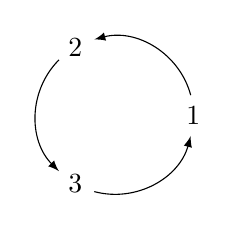
\begin{tikzpicture}
	\def \n {3}
	\def \radius {1cm}
	\def \margin {15} 
	\foreach \s in {1,...,\n}
	{
 	 \node at ({360/\n * (\s - 1)}:\radius) {$\s$};
	  \draw[->, >=latex] ({360/\n * (\s - 1)+\margin}:\radius) 
 	   arc ({360/\n * (\s - 1)+\margin}:{360/\n * (\s)-\margin}:\radius);
	}
	\end{tikzpicture}$\\
	This is read 1 goes to 2; 2 goes to 3; and 3 goes to 1.
	\item
	Cycle notation: $(123)$\\
	This is also read as 1 goes to 2; 2 goes to 3; and 3 goes to 1.
	\end{itemize}
Changing from one to another is very important and therefore there are many exercises listed in competencies.
\item
The length of a cycle is equal to the number of elements in the cycle, i.e. how many elements are inside the parentheses. (Definiton~\ref{cycle_length})
\item
The  identity permutation $\var{id}$ may be conceived of as a cycle of length 0 (or ``empty cycle'').
\item
Cycle notation does not specify the domain (which is determined by the context).  For example, the cycle $(243)$ is a cycle in $S_4$ that leaves  1 fixed ,but it is also a cycle in $S_6$ that leaves 1,5, 6 fixed. (Warning~\ref{cycle_domain})
\item
Composition of cycles = product of cycles, i.e.  $\sigma \compose \tau$ = $\sigma \tau$
\item
Composition/product of cycles is always right to left
\item
Disjoint cycles are cycles which share no common elements.  (Definition~\ref{disjoint_cycles})
\item
Disjoint cycles commute, which means they can be composed in any order and produce the same product. (Proposition~\ref{proposition:Permutations:disjoint_cycles_commute}
\item
Every permutation in a symmetric group, $S_n$, can be written as $\var{id}$, a single cycle, or as the product of disjoint cycles. (Proposition~\ref{proposition:Permutations:perm_simple_notation})
\end{enumerate}

\subsubsection*{Competencies}
\begin{enumerate}
\item
Write cycles using the different notations.  (Ex. \ref{exercise:Permutations:equal_cycles2}, \ref{exercise:Permutations:equal_cycles1},  \ref{exercise:Permutations:long_cycle_perm1}, \ref{exercise:Permutations:long_cycle_perm2}, \ref{exercise:Permutations:long_cycle_perm3}, \ref{exercise:Permutations:short_cycle1}, \ref{exercise:Permutations:short_cycle2}, \ref{exercise:Permutations:tab_to_cycle}, \ref{exercise:Permutations:cycle_to_tab})
\item
Find the product of cycles.  (Ex. \ref{exercise:Permutations:cycle_comp_exer1}, \ref{exercise:Permutations:cycle_comp_5}, \ref{exercise:Permutations:cycle_comp_2})
\item
Determine whether or not cycles commute (Ex. \ref{exercise:Permutations:perm_not_comm}, \ref{exercise:Permutations:dis_cycles_comm})
\item
Determine all cycle structures of permutations in a given $S_n$. (Ex. \ref{exercise:Permutations:cycle_types})
\end{enumerate}


\subsection*{Section \ref{algebraic_props}, Algebraic properties of cycles}
\subsubsection*{Concepts:}
\begin{enumerate}
\item
Notation: $\sigma^n$ is the permutation obtained by composing $\sigma$ with itself $n$ times.
\item
The order of a cycle, $\sigma$, is the smallest $k \in {\mathbb N}$ s.t. $\sigma^k = id$.  The order of a cycle is always equal to the cycle's length, so $k$ is always the length of the cycle. (Definition~\ref{def_order_cycle}, Proposition~\ref{proposition:Permutations:order_of_cycle})
\item
If two cycles are disjoint, then the order of the product of those cycles is the least common multiple (lcm) of the order of each individual cycle, i.e. $|\sigma \tau|$ = lcm$(|\sigma|, |\tau|)$ (Proposition~\ref{proposition:Permutations:order_of_2disjoint_cycles})
\item
A \term*{transposition}\index{Permutation!transposition}\index{Transposition!permutation} is a cycle of length 2. (Definition~\ref{Transposition})
\item
Any cycle may be expressed as the product of transpositions ( Proposition~\ref{proposition:Permutations:transposition_formula}).
\item
Any permutation may be expressed as the product of transpositions ( Proposition~\ref{proposition:Permutations:trans_perm}).
\item
For any transposition $\tau$, $\tau^{-1} = \tau$ (Proposition~\ref{proposition:Permutations:trans_inv}.
\item
For any cycle, the inverse of the cycle is the first element in the cycle, followed by the remaining elements written in reverse order Proposition~\ref{proposition:Permutations:cycle_inv}.
\end{enumerate}

\subsubsection*{Competencies}
\begin{enumerate}
\item
Compute powers of cycles. (Ex. \ref{exercise:Permutations:4th_power}, \ref{exercise:Permutations:6th_power}, \ref{exercise:Permutations:cycle_order_1}, \ref{exercise:Permutations:disjoint_order_1})
\item
Compute powers of permutations. (Ex. \ref{exercise:Permutations:power of n-cycle1}, \ref{exercise:Permutations:length_equals_order2})
\item
Give step-by-step justification for the calculation of the composition of permutations. (Example~\ref{example:Permutations:disjoint_squared},  Ex. \ref{exercise:Permutations:disjoint_cube}, \ref{exercise:Permutations:k_power_disjoint_cycles})
\item
Find the order of permutations based on their cycle structure. (Ex. \ref{exercise:Permutations:Sn_orders}, \ref{exercise:Permutations:disjoint_order_2})
\item
Be able to write a produt of disjoint cycles as a product of transpositons, and vice versa (Ex. \ref{exercise:Permutations:example_transpositions}, \ref{exercise:Permutations:example_transpositions2}, \ref{exercise:Permutations:prod_of_trans_1}, \ref{exercise:Permutations:prod_of_trans_1}, \ref{exercise:Permutations:prod_of_trans_2})
\item
Compute inverses of permutations written as products of cycles (Ex. \ref{exercise:Permutations:inv_comps})
\end{enumerate}


\subsection*{Section \ref{sec:Permutations:OtherGroups}, Other groups of permutations}
\subsubsection*{Concepts:}
\begin{enumerate}
\item 
Cycles change structure when  multiplied by transposition $(ab)$, depending on where $a$ and $b$ are in the original cycle. (Figure~\ref{fig:abC} and  Figure~\ref{fig:abC2})
\item
The \term*{parity} of a permutation $\sigma$ is determined by mod(sum of cycle lengths minus number of cycles, 2). Parity 0 is referred to as \term*{even}, and parity 1 as \term*{odd}. (Definition~\ref{def_parity})
\item
Multiplication by a transposition changes the parity of a permutation. (Proposition~\ref{proposition:Permutations:multByTrans})
\item
A permutation is even (resp. odd) if and only if it can be expressed as the product of an even (resp. odd) number of transpositions (Proposition~\ref{proposition:Permutations:even_and_odd}).
\item
Cycles with even (resp. odd) length are odd (resp. even) permutations (Exercise~\ref{exercise:Permutations:even_odd}).
\end{enumerate}

\subsubsection*{Competencies}
\begin{enumerate}
\item
 Determine how multiplying a permutation by a transposition changes the cycle structure and number of cycles in a  permutation.  (Ex. \ref{exercise:Permutations:trans_perm}. \ref{exercise:Permutations:trans_perm2})
\item
Determine whether permutations are even or odd, according to their cycle structure (Ex. \ref{exercise:Permutations:even_odd},  \ref{exercise:Permutations:Sn_even_odd}),
\item
Write proofs of parity properties. (Ex. \ref{exercise:Permutations:Ex95})
\end{enumerate}
%\subsection*{Section \ref{}, }
%\subsubsection*{Concepts:}
%\begin{enumerate}
%\item 
%
%\item
%
%\item
%
%\item
%
%\end{enumerate}
%
%\subsubsection*{Competencies}
%\begin{enumerate}
%\item
%
%\item
%
%\item
%
%\end{enumerate}





